\documentclass{article}
\usepackage{amssymb,amsmath}
\usepackage{ifxetex,ifluatex}
\ifxetex
  \usepackage{fontspec,xltxtra,xunicode}
  \defaultfontfeatures{Mapping=tex-text,Scale=MatchLowercase}
\else
  \ifluatex
    \usepackage{fontspec}
    \defaultfontfeatures{Mapping=tex-text,Scale=MatchLowercase}
  \else
    \usepackage[utf8]{inputenc}
  \fi
\fi
\usepackage{ctable}
\usepackage{float} % provides the H option for float placement
\usepackage{graphicx}
% We will generate all images so they have a width \maxwidth. This means
% that they will get their normal width if they fit onto the page, but
% are scaled down if they would overflow the margins.
\makeatletter
\def\maxwidth{\ifdim\Gin@nat@width>\linewidth\linewidth
\else\Gin@nat@width\fi}
\makeatother
\let\Oldincludegraphics\includegraphics
\renewcommand{\includegraphics}[1]{\Oldincludegraphics[width=\maxwidth]{#1}}
\ifxetex
  \usepackage[setpagesize=false, % page size defined by xetex
              unicode=false, % unicode breaks when used with xetex
              xetex]{hyperref}
\else
  \usepackage[unicode=true]{hyperref}
\fi
\hypersetup{breaklinks=true, pdfborder={0 0 0}}
\setlength{\parindent}{0pt}
\setlength{\parskip}{6pt plus 2pt minus 1pt}
\setlength{\emergencystretch}{3em}  % prevent overfull lines
\setcounter{secnumdepth}{0}

\title{Descriptives}
\author{(Username not set) (E-mail address not set)}
\date{2011--04--26 20:25 CET}

\begin{document}
\maketitle

\subsection{Description}

This template will return descriptive statistics of numerical, or
frequency tables of categorical variables.

\subsubsection{\emph{gender} (``Gender'')}

The dataset has 709 observations with 709 valid values (missing: 0) in
\emph{gender} (``Gender''). This variable seems to be a factor.

\paragraph{Base statistics}

\ctable[pos = H, center, botcap]{lllll}
{% notes
}
{% rows
\FL
\textbf{gender} & \textbf{N} & \textbf{pct} & \textbf{cum.n} & \textbf{cum.pct}
\ML
male & 7344.00 & 60.93 & 7344.00 & 60.93
\\\noalign{\medskip}
female & 4709.00 & 39.07 & 12053.00 & 100.00
\LL
}

\paragraph{Barplot}

\begin{figure}[htbp]
\centering
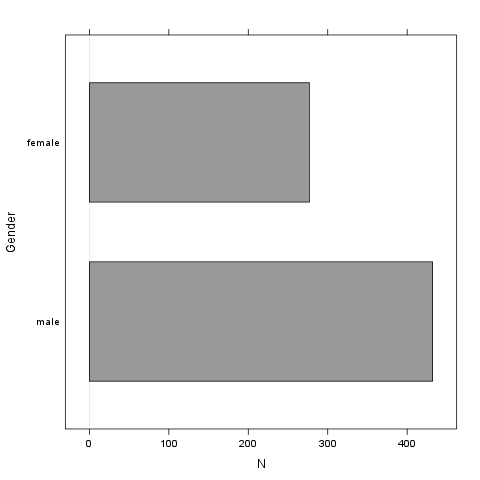
\includegraphics{2a42fb1eb44bf1361b44216c6b0c16ee.png}
\caption{}
\end{figure}

It seems that the highest value is 2 which is exactly 2 times higher
than the smallest value (1).

\subsubsection{\emph{age} (``Age'')}

The dataset has 709 observations with 709 valid values (missing: 0) in
\emph{age} (``Age''). This variable seems to be numeric.

\paragraph{Base statistics}

\ctable[pos = H, center, botcap]{llll}
{% notes
}
{% rows
\FL
\textbf{value} & \textbf{mean} & \textbf{sd} & \textbf{var}
\ML
(all) & 24.56 & 6.84 & 46.78
\LL
}

\paragraph{Histogram}

\begin{figure}[htbp]
\centering
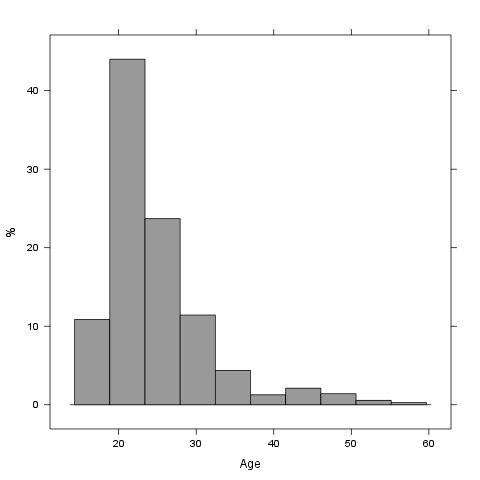
\includegraphics{76fc57f9d2387aff730be60323f25624.png}
\caption{}
\end{figure}

It seems that the highest value is 58 which is exactly 3.625 times
higher than the smallest value (16).

The standard deviation is 6.8399 (variance: 46.784). The expected value
is around 24.557, somewhere between 24.054 and 25.061 (SE: 0.2569).

If we suppose that \emph{Age} is not near to a normal distribution
(test: , skewness: 1.9568, kurtosis: 7.6428), checking the median (23)
might be a better option instead of the mean. The interquartile range
(6) measures the statistics dispersion of the variable (similar to
standard deviation) based on median.

\subsection{Description}

This template will return descriptive statistics of numerical, or
frequency tables of categorical variables.

\subsubsection{\emph{chatim} (``Chat \& IM usage'')}

The dataset has 709 observations with 709 valid values (missing: 0) in
\emph{chatim} (``Chat \& IM usage''). This variable seems to be a
factor.

\paragraph{Base statistics}

\ctable[pos = H, center, botcap]{lllll}
{% notes
}
{% rows
\FL
\textbf{chatim} & \textbf{N} & \textbf{pct} & \textbf{cum.n} & \textbf{cum.pct}
\ML
never & 896.00 & 9.03 & 896.00 & 9.03
\\\noalign{\medskip}
very rarely & 1092.00 & 11.00 & 1988.00 & 20.03
\\\noalign{\medskip}
rarely & 910.00 & 9.17 & 2898.00 & 29.20
\\\noalign{\medskip}
sometimes & 1736.00 & 17.49 & 4634.00 & 46.69
\\\noalign{\medskip}
often & 1988.00 & 20.03 & 6622.00 & 66.71
\\\noalign{\medskip}
very often & 1316.00 & 13.26 & 7938.00 & 79.97
\\\noalign{\medskip}
always & 1988.00 & 20.03 & 9926.00 & 100.00
\LL
}

\textbf{Warning} in ``if (is.numeric(var)) \{ ; rp.desc(NULL,
rp.name(var), c(`mean', `sd', `var'), rp.data) ; \} else \{ ;
rp.freq(rp.name(var), rp.data) ; \}'': ``invalid factor level, NAs
generated + invalid factor level, NAs generated + invalid factor level,
NAs generated''

\paragraph{Barplot}

\begin{figure}[htbp]
\centering
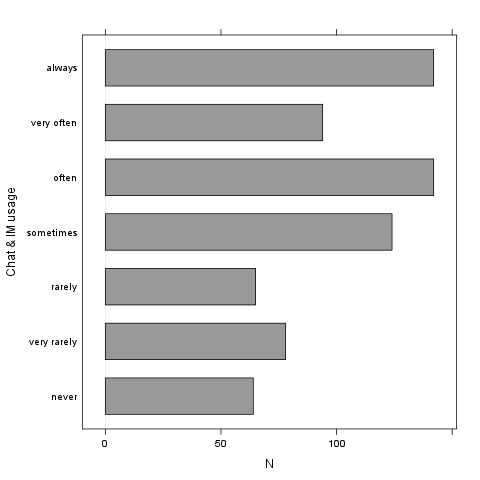
\includegraphics{18ee2d4410677e2bbc343a9a4889cc97.png}
\caption{}
\end{figure}

It seems that the highest value is 7 which is exactly 7 times higher
than the smallest value (1).

\subsubsection{\emph{game} (``On-line games usage'')}

The dataset has 709 observations with 709 valid values (missing: 0) in
\emph{game} (``On-line games usage''). This variable seems to be a
factor.

\paragraph{Base statistics}

\ctable[pos = H, center, botcap]{lllll}
{% notes
}
{% rows
\FL
\textbf{game} & \textbf{N} & \textbf{pct} & \textbf{cum.n} & \textbf{cum.pct}
\ML
never & 5152.00 & 51.90 & 5152.00 & 51.90
\\\noalign{\medskip}
very rarely & 1848.00 & 18.62 & 7000.00 & 70.52
\\\noalign{\medskip}
rarely & 490.00 & 4.94 & 7490.00 & 75.46
\\\noalign{\medskip}
sometimes & 910.00 & 9.17 & 8400.00 & 84.63
\\\noalign{\medskip}
often & 532.00 & 5.36 & 8932.00 & 89.99
\\\noalign{\medskip}
very often & 518.00 & 5.22 & 9450.00 & 95.20
\\\noalign{\medskip}
always & 476.00 & 4.80 & 9926.00 & 100.00
\LL
}

\textbf{Warning} in ``if (is.numeric(var)) \{ ; rp.desc(NULL,
rp.name(var), c(`mean', `sd', `var'), rp.data) ; \} else \{ ;
rp.freq(rp.name(var), rp.data) ; \}'': ``invalid factor level, NAs
generated + invalid factor level, NAs generated + invalid factor level,
NAs generated''

\paragraph{Barplot}

\begin{figure}[htbp]
\centering
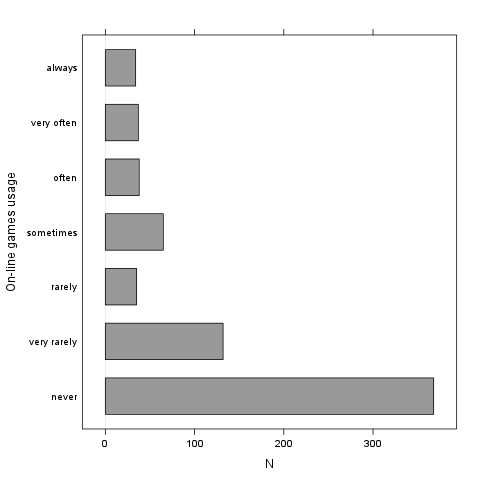
\includegraphics{db92f166fe1966dbd5c6f0b909c181b2.png}
\caption{}
\end{figure}

It seems that the highest value is 7 which is exactly 7 times higher
than the smallest value (1).

\subsubsection{\emph{surf} (``Web surfing usage'')}

The dataset has 709 observations with 709 valid values (missing: 0) in
\emph{surf} (``Web surfing usage''). This variable seems to be a factor.

\paragraph{Base statistics}

\ctable[pos = H, center, botcap]{lllll}
{% notes
}
{% rows
\FL
\textbf{surf} & \textbf{N} & \textbf{pct} & \textbf{cum.n} & \textbf{cum.pct}
\ML
never & 238.00 & 2.40 & 238.00 & 2.40
\\\noalign{\medskip}
very rarely & 364.00 & 3.67 & 602.00 & 6.06
\\\noalign{\medskip}
rarely & 476.00 & 4.80 & 1078.00 & 10.86
\\\noalign{\medskip}
sometimes & 1624.00 & 16.36 & 2702.00 & 27.22
\\\noalign{\medskip}
often & 2296.00 & 23.13 & 4998.00 & 50.35
\\\noalign{\medskip}
very often & 2114.00 & 21.30 & 7112.00 & 71.65
\\\noalign{\medskip}
always & 2814.00 & 28.35 & 9926.00 & 100.00
\LL
}

\textbf{Warning} in ``if (is.numeric(var)) \{ ; rp.desc(NULL,
rp.name(var), c(`mean', `sd', `var'), rp.data) ; \} else \{ ;
rp.freq(rp.name(var), rp.data) ; \}'': ``invalid factor level, NAs
generated + invalid factor level, NAs generated + invalid factor level,
NAs generated''

\paragraph{Barplot}

\begin{figure}[htbp]
\centering
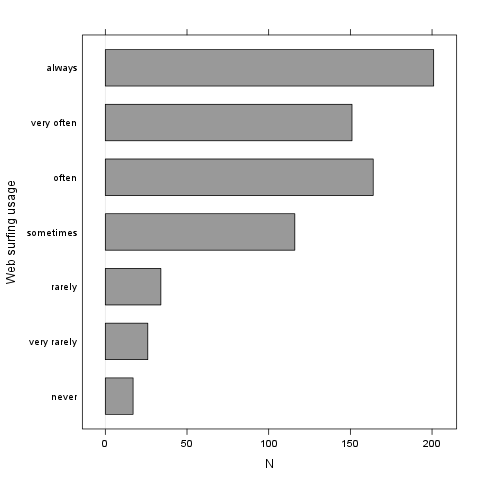
\includegraphics{42a485477f7c7e629c55f3f106b2f482.png}
\caption{}
\end{figure}

It seems that the highest value is 7 which is exactly 7 times higher
than the smallest value (1).

\subsubsection{\emph{email} (``Email usage'')}

The dataset has 709 observations with 709 valid values (missing: 0) in
\emph{email} (``Email usage''). This variable seems to be a factor.

\paragraph{Base statistics}

\ctable[pos = H, center, botcap]{lllll}
{% notes
}
{% rows
\FL
\textbf{email} & \textbf{N} & \textbf{pct} & \textbf{cum.n} & \textbf{cum.pct}
\ML
never & 182.00 & 1.83 & 182.00 & 1.83
\\\noalign{\medskip}
very rarely & 532.00 & 5.36 & 714.00 & 7.19
\\\noalign{\medskip}
rarely & 714.00 & 7.19 & 1428.00 & 14.39
\\\noalign{\medskip}
sometimes & 1260.00 & 12.69 & 2688.00 & 27.08
\\\noalign{\medskip}
often & 1806.00 & 18.19 & 4494.00 & 45.28
\\\noalign{\medskip}
very often & 1624.00 & 16.36 & 6118.00 & 61.64
\\\noalign{\medskip}
always & 3808.00 & 38.36 & 9926.00 & 100.00
\LL
}

\textbf{Warning} in ``if (is.numeric(var)) \{ ; rp.desc(NULL,
rp.name(var), c(`mean', `sd', `var'), rp.data) ; \} else \{ ;
rp.freq(rp.name(var), rp.data) ; \}'': ``invalid factor level, NAs
generated + invalid factor level, NAs generated + invalid factor level,
NAs generated''

\paragraph{Barplot}

\begin{figure}[htbp]
\centering
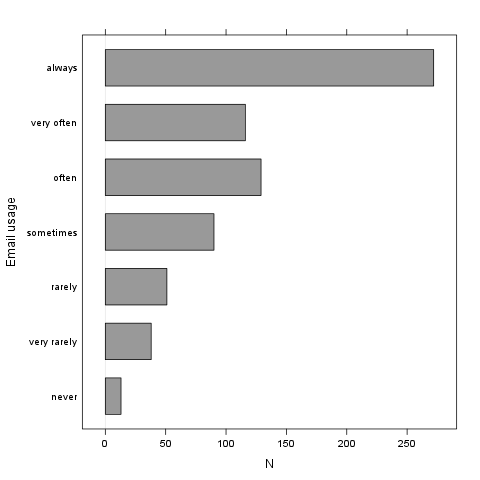
\includegraphics{4271956be974e19ffa2034d316fd201c.png}
\caption{}
\end{figure}

It seems that the highest value is 7 which is exactly 7 times higher
than the smallest value (1).

\subsubsection{\emph{download} (``Download usage'')}

The dataset has 709 observations with 709 valid values (missing: 0) in
\emph{download} (``Download usage''). This variable seems to be a
factor.

\paragraph{Base statistics}

\ctable[pos = H, center, botcap]{lllll}
{% notes
}
{% rows
\FL
\textbf{download} & \textbf{N} & \textbf{pct} & \textbf{cum.n} & \textbf{cum.pct}
\ML
never & 154.00 & 1.55 & 154.00 & 1.55
\\\noalign{\medskip}
very rarely & 406.00 & 4.09 & 560.00 & 5.64
\\\noalign{\medskip}
rarely & 420.00 & 4.23 & 980.00 & 9.87
\\\noalign{\medskip}
sometimes & 1190.00 & 11.99 & 2170.00 & 21.86
\\\noalign{\medskip}
often & 1820.00 & 18.34 & 3990.00 & 40.20
\\\noalign{\medskip}
very often & 2394.00 & 24.12 & 6384.00 & 64.32
\\\noalign{\medskip}
always & 3542.00 & 35.68 & 9926.00 & 100.00
\LL
}

\textbf{Warning} in ``if (is.numeric(var)) \{ ; rp.desc(NULL,
rp.name(var), c(`mean', `sd', `var'), rp.data) ; \} else \{ ;
rp.freq(rp.name(var), rp.data) ; \}'': ``invalid factor level, NAs
generated + invalid factor level, NAs generated + invalid factor level,
NAs generated''

\paragraph{Barplot}

\begin{figure}[htbp]
\centering
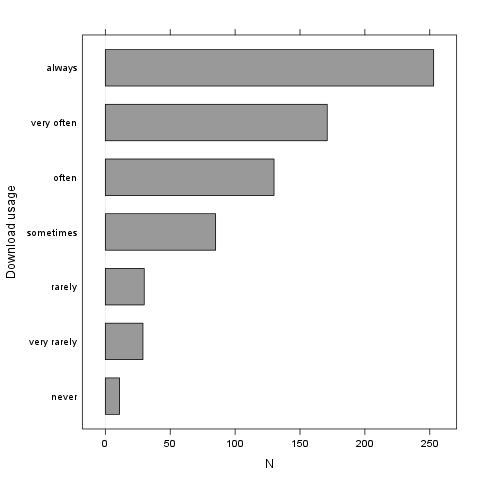
\includegraphics{ec8a2289e719ec679a4abc2f1b3a62ec.png}
\caption{}
\end{figure}

It seems that the highest value is 7 which is exactly 7 times higher
than the smallest value (1).

\subsubsection{\emph{forum} (``Web forums usage'')}

The dataset has 709 observations with 709 valid values (missing: 0) in
\emph{forum} (``Web forums usage''). This variable seems to be a factor.

\paragraph{Base statistics}

\ctable[pos = H, center, botcap]{lllll}
{% notes
}
{% rows
\FL
\textbf{forum} & \textbf{N} & \textbf{pct} & \textbf{cum.n} & \textbf{cum.pct}
\ML
never & 1120.00 & 11.28 & 1120.00 & 11.28
\\\noalign{\medskip}
very rarely & 1176.00 & 11.85 & 2296.00 & 23.13
\\\noalign{\medskip}
rarely & 1036.00 & 10.44 & 3332.00 & 33.57
\\\noalign{\medskip}
sometimes & 1736.00 & 17.49 & 5068.00 & 51.06
\\\noalign{\medskip}
often & 1568.00 & 15.80 & 6636.00 & 66.85
\\\noalign{\medskip}
very often & 1750.00 & 17.63 & 8386.00 & 84.49
\\\noalign{\medskip}
always & 1540.00 & 15.51 & 9926.00 & 100.00
\LL
}

\textbf{Warning} in ``if (is.numeric(var)) \{ ; rp.desc(NULL,
rp.name(var), c(`mean', `sd', `var'), rp.data) ; \} else \{ ;
rp.freq(rp.name(var), rp.data) ; \}'': ``invalid factor level, NAs
generated + invalid factor level, NAs generated + invalid factor level,
NAs generated''

\paragraph{Barplot}

\begin{figure}[htbp]
\centering
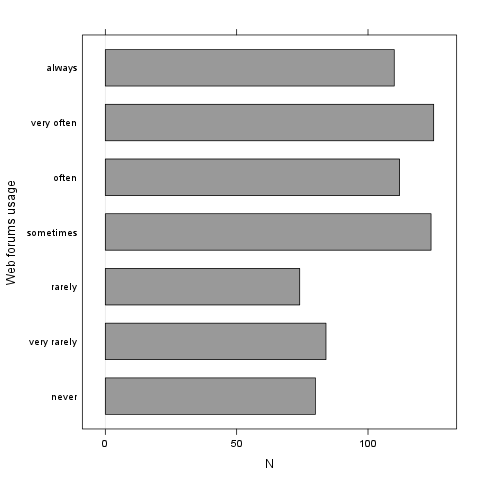
\includegraphics{3f14c76d2ae5a41c21a771f3fd794ca3.png}
\caption{}
\end{figure}

It seems that the highest value is 7 which is exactly 7 times higher
than the smallest value (1).

\subsubsection{\emph{socnet} (``Social networks usage'')}

The dataset has 709 observations with 709 valid values (missing: 0) in
\emph{socnet} (``Social networks usage''). This variable seems to be a
factor.

\paragraph{Base statistics}

\ctable[pos = H, center, botcap]{lllll}
{% notes
}
{% rows
\FL
\textbf{socnet} & \textbf{N} & \textbf{pct} & \textbf{cum.n} & \textbf{cum.pct}
\ML
never & 2940.00 & 29.62 & 2940.00 & 29.62
\\\noalign{\medskip}
very rarely & 1554.00 & 15.66 & 4494.00 & 45.28
\\\noalign{\medskip}
rarely & 826.00 & 8.32 & 5320.00 & 53.60
\\\noalign{\medskip}
sometimes & 1316.00 & 13.26 & 6636.00 & 66.85
\\\noalign{\medskip}
often & 1148.00 & 11.57 & 7784.00 & 78.42
\\\noalign{\medskip}
very often & 1190.00 & 11.99 & 8974.00 & 90.41
\\\noalign{\medskip}
always & 952.00 & 9.59 & 9926.00 & 100.00
\LL
}

\textbf{Warning} in ``if (is.numeric(var)) \{ ; rp.desc(NULL,
rp.name(var), c(`mean', `sd', `var'), rp.data) ; \} else \{ ;
rp.freq(rp.name(var), rp.data) ; \}'': ``invalid factor level, NAs
generated + invalid factor level, NAs generated + invalid factor level,
NAs generated''

\paragraph{Barplot}

\begin{figure}[htbp]
\centering
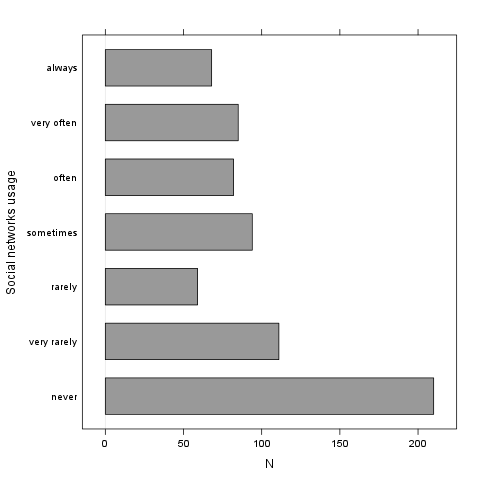
\includegraphics{c1a552be1b3a4299ff06e272129d8096.png}
\caption{}
\end{figure}

It seems that the highest value is 7 which is exactly 7 times higher
than the smallest value (1).

\subsubsection{\emph{xxx} (``Adult sites usage'')}

The dataset has 709 observations with 709 valid values (missing: 0) in
\emph{xxx} (``Adult sites usage''). This variable seems to be a factor.

\paragraph{Base statistics}

\ctable[pos = H, center, botcap]{lllll}
{% notes
}
{% rows
\FL
\textbf{xxx} & \textbf{N} & \textbf{pct} & \textbf{cum.n} & \textbf{cum.pct}
\ML
never & 4102.00 & 41.33 & 4102.00 & 41.33
\\\noalign{\medskip}
very rarely & 1792.00 & 18.05 & 5894.00 & 59.38
\\\noalign{\medskip}
rarely & 770.00 & 7.76 & 6664.00 & 67.14
\\\noalign{\medskip}
sometimes & 1918.00 & 19.32 & 8582.00 & 86.46
\\\noalign{\medskip}
often & 672.00 & 6.77 & 9254.00 & 93.23
\\\noalign{\medskip}
very often & 406.00 & 4.09 & 9660.00 & 97.32
\\\noalign{\medskip}
always & 266.00 & 2.68 & 9926.00 & 100.00
\LL
}

\textbf{Warning} in ``if (is.numeric(var)) \{ ; rp.desc(NULL,
rp.name(var), c(`mean', `sd', `var'), rp.data) ; \} else \{ ;
rp.freq(rp.name(var), rp.data) ; \}'': ``invalid factor level, NAs
generated + invalid factor level, NAs generated + invalid factor level,
NAs generated''

\paragraph{Barplot}

\begin{figure}[htbp]
\centering
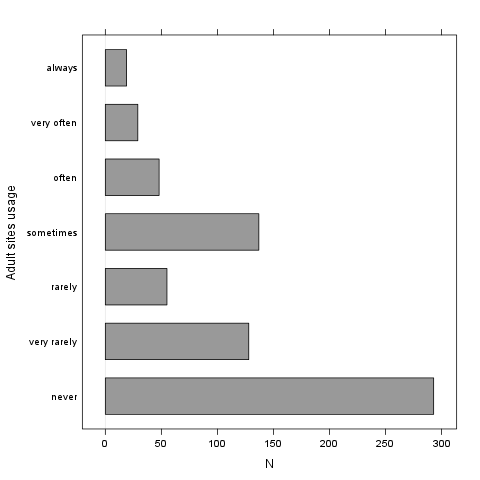
\includegraphics{053614b5b842759f559adcc0da8cc645.png}
\caption{}
\end{figure}

It seems that the highest value is 7 which is exactly 7 times higher
than the smallest value (1).

\subsubsection{\emph{long.use} (``How long you've been on the
Internet?'')}

The dataset has 709 observations with 709 valid values (missing: 0) in
\emph{long.use} (``How long you've been on the Internet?''). This
variable seems to be a factor.

\paragraph{Base statistics}

\ctable[pos = H, center, botcap]{lllll}
{% notes
}
{% rows
\FL
\textbf{long.use} & \textbf{N} & \textbf{pct} & \textbf{cum.n} & \textbf{cum.pct}
\ML
less than 6 months & 294.00 & 2.96 & 294.00 & 2.96
\\\noalign{\medskip}
1 years & 728.00 & 7.33 & 1022.00 & 10.30
\\\noalign{\medskip}
2 years & 966.00 & 9.73 & 1988.00 & 20.03
\\\noalign{\medskip}
3 years & 1092.00 & 11.00 & 3080.00 & 31.03
\\\noalign{\medskip}
4 years & 1064.00 & 10.72 & 4144.00 & 41.75
\\\noalign{\medskip}
5 years & 1036.00 & 10.44 & 5180.00 & 52.19
\\\noalign{\medskip}
5 years and more & 4746.00 & 47.81 & 9926.00 & 100.00
\LL
}

\textbf{Warning} in ``if (is.numeric(var)) \{ ; rp.desc(NULL,
rp.name(var), c(`mean', `sd', `var'), rp.data) ; \} else \{ ;
rp.freq(rp.name(var), rp.data) ; \}'': ``invalid factor level, NAs
generated + invalid factor level, NAs generated + invalid factor level,
NAs generated''

\paragraph{Barplot}

\begin{figure}[htbp]
\centering
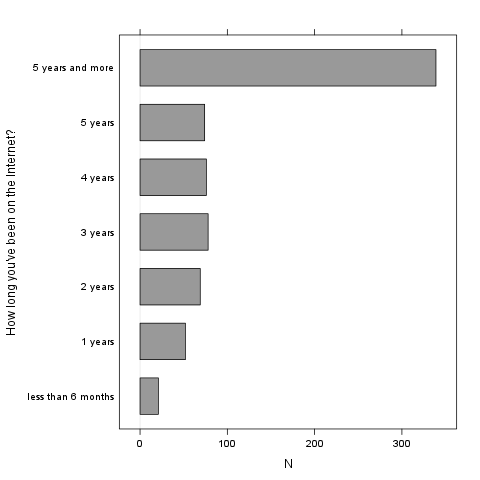
\includegraphics{ac7f8b3e1fb841eb17beaceee8e09dd1.png}
\caption{}
\end{figure}

It seems that the highest value is 7 which is exactly 7 times higher
than the smallest value (1).

\end{document}
